\documentclass{article}

% Double-blind main-track submission.
\usepackage[preprint]{neurips_2026}

\usepackage[utf8]{inputenc}
\usepackage[T1]{fontenc}
\usepackage{hyperref}
\usepackage{url}
\usepackage{booktabs}
\usepackage{amsfonts}
\usepackage{amsmath}
\usepackage{graphicx}
\usepackage{xcolor}
\usepackage{microtype}
\usepackage{multirow}

% Visible placeholder macro for numbers pending experiment completion.
% Final submission: audit \TODO and replace each with real values.
\newcommand{\TODO}[1]{\textcolor{red}{\textbf{[TODO: #1]}}}

\title{How Foveated Vision Shapes Cognitive Maps in Navigation Agents}

\author{%
  Anonymous authors\\
  Paper under double-blind review\\
}

\begin{document}
\maketitle

\begin{abstract}
Animal spatial cognition is built on eccentricity-dependent visual acuity: primates see sharply only within $\sim$2\textdegree{} of gaze, yet their hippocampi code joint place--view--action state~\citep{wirth2017gaze,rolls2024why}. Map-like representations also emerge in the recurrent memories of artificial navigation agents, but only under conditions of blind or spatially uniform perception~\citep{wijmans2023emergence}. How does the format of learned spatial memory change when the sensor is foveated rather than uniform, and when the gaze that directs foveation is learned rather than fixed? We train navigation agents in Habitat under five visual conditions---blind, uniform, foveated (fixed centre), matched-compute, and foveated (learned gaze)---and analyse the resulting recurrent memory with linear probes, cross-condition CKA, probe transfer, per-unit spatial-information measures, and two behavioural interventions directly on the recurrent state (memory transplant and shortcut discovery). Three findings emerge, each with a biological precedent. \emph{(1)~Compensatory memory.} Spatially non-uniform vision induces longer-lived spatial traces: the foveated agent retains decodable position information five steps into the past ($R^2=0.56$) while the uniform baseline's probe collapses ($R^2=-1.5$) --- the learned-agent analog of compensatory hippocampal coupling in blind humans~\citep{kupers2014blind} and grid-cell collapse in darkness~\citep{chen2016grid}. \emph{(2)~Sensor-dependent representational format.} Each visual condition produces a distinct representational geometry (CKA $<0.004$ between all pairs; catastrophic probe transfer) despite $>97\%$ task success; pasting a donor's mid-episode hidden state into a different-condition recipient drops SPL by up to $0.21$ even between the two foveated variants, mirroring the hippocampal remapping that occurs when bats switch between vision and echolocation~\citep{geva2016remapping}. \emph{(3)~Gaze-locked representational content.} The learned-gaze agent collapses to a near-constant gaze and, as a result, builds a content-shifted representation: highest compass decoding of any condition ($R^2=0.94$) but near-chance GPS decoding ($R^2=0.03$); carrying memory across episodes with a new goal hurts it least ($15\%$ relative SPL drop vs.\ $41$--$52\%$ for uniform/blind). This is consistent with the biological evidence that each saccade is a memory-encoding event~\citep{jutras2013saccades,tas2016overt}: a gaze restricted to one scene region restricts memory to what that region reliably carries, here heading rather than position. Together these establish sensor structure and gaze policy as causal factors in the format of learned spatial memory, and add a controlled instance to the comparative-neuroscience evidence that modality and gaze shape where and how spatial information is held internally.
\end{abstract}


\section{Introduction}

Decades of animal-navigation research rest on a specific observation: what an animal foveates determines what its hippocampus encodes. Wirth et al.~\citep{wirth2017gaze} showed that primate hippocampal cells represent not just location but a joint code of place, view, and task context; Rolls~\citep{rolls2024why} argued that the primate fovea is precisely why primates have \emph{spatial-view cells} while rats, with their near-panoramic retinae, have \emph{place cells}. Geva-Sagiv et al.~\citep{geva2016remapping} extended the claim within a single animal: the same bat, in the same environment, produces non-overlapping hippocampal populations when it alternates between vision and echolocation, so sensor modality reshapes representational format rather than merely scaling its strength. Yet when map-like representations have been shown to emerge in the recurrent memories of artificial navigation agents~\citep{wijmans2023emergence}, it has always been under conditions of blind or spatially uniform perception---conditions no visual animal experiences. We ask the question that cross-species and cross-modality comparisons cannot cleanly isolate: when sensor structure is the only free variable, does the format of learned spatial memory change with it?

Two accounts make divergent predictions for a foveated agent. A \emph{passive buffering} memory stores whatever it currently perceives; its decodable content should \emph{fall} in quality when current input is degraded and persist only as long as the visual snapshot is fresh. A \emph{compensatory} memory does the opposite: when current input is unreliable, it \emph{invests} in internal state to cover the gap, so decodable content should persist over longer temporal horizons than for an agent whose current input is always reliable. The biological precedent favours the compensatory pattern: congenitally blind humans develop enhanced hippocampal coupling with sensory and occipital cortices and outperform sighted controls on non-visual spatial-working-memory tasks~\citep{kupers2014blind}, and rodent grid-cell periodicity collapses in darkness despite preserved head-direction inputs~\citep{chen2016grid}. Our central question is whether the learned-agent analog follows the same pattern.

We test three hypotheses, each with an explicit prediction and a biological precedent. \textbf{H1 (Compensatory memory).} Foveated agents should retain spatial information over longer temporal horizons than uniformly-sighted agents---the learned-agent analog of compensatory hippocampal coupling in blind humans~\citep{kupers2014blind} and grid-cell collapse under impoverished visual input~\citep{chen2016grid}. Signature: retrospective spatial-memory probe $R^2$ at lag $k$ stays high for foveated and drops for uniform. \textbf{H2 (Representational divergence).} Foveation should produce a representation format distinct from a uniform code rather than a degraded version of it, mirroring the format-level divergences observed across sensory modalities within animals~\citep{geva2016remapping} and between primate and rodent hippocampi~\citep{rolls2024why}. Signature: cross-condition CKA near zero, probe weights failing to transfer across conditions, while within-condition probes succeed. \textbf{H3 (Epistemic gaze).} When gaze is learned end-to-end through the navigation loss, it should target regions where memory is most uncertain, consistent with the ideal-observer formulation of visual search~\citep{najemnik2005optimal,gottlieb2013information} and with the evidence that overt saccades are themselves memory-encoding events~\citep{jutras2013saccades,tas2016overt}. Signature: correlation between the learned-gaze coordinate and per-step position-probe residual on the fixed-gaze variant.

\paragraph{Findings.}
H1 and H2 are supported by clean large-magnitude effects (path-history $R^2=0.56$ at lag 5 for foveated vs.\ $-1.53$ for uniform; cross-condition CKA $<0.004$ on every pair). H3 in its strong form is \emph{not} supported: the learned-gaze decoder converges to a near-constant output, and two anti-collapse regularisers restore gaze variance only at the cost of task performance. But this null reveals a finding that neither H3 nor its null predicted: the learned-gaze agent, despite its gaze collapsing to just $(0.49,0.62)$, exhibits a \emph{categorical} representational shift --- the strongest compass encoding of any condition ($R^2=0.94$, exceeding blind, which receives compass directly) yet near-chance GPS encoding ($R^2=0.03$), at every LSTM layer. Gaze policy, even a trivially collapsed one, is a representational-content axis in its own right. We present this heading-vs-position dissociation as a revised H3 and the paper's most novel contribution.


\section{Related Work}

\paragraph{Cognitive maps in biological navigation.}
Tolman~\citep{tolman1948cognitive} introduced the notion of a ``cognitive map''; Epstein et al.~\citep{epstein2017cognitive} operationalise it as a unified representation of the spatial environment supporting memory and future action, instantiated in place, grid, border, and head-direction cells. Bellmund et al.~\citep{bellmund2018navigating} and Behrens et al.~\citep{behrens2018cognitive} generalise the construct to relational maps beyond Euclidean space, and Peer et al.~\citep{peer2021cognitive} distinguish continuous cognitive \emph{maps} from discrete cognitive \emph{graphs}. Two results in this literature directly anchor our hypotheses. Wirth et al.~\citep{wirth2017gaze} showed that primate hippocampal cells code joint place--view--action state; Rolls~\citep{rolls2024why,rolls2023viewcells} argues that primate \emph{spatial-view cells} and rat \emph{place cells} reflect the different sampling statistics of foveated versus near-panoramic vision. Geva-Sagiv et al.~\citep{geva2016remapping} observed format-level hippocampal remapping when the same bat alternates between vision and echolocation, a within-animal analog of our across-condition comparison.

\paragraph{Active vision and memory formation.}
In everyday behaviour, gaze is overwhelmingly task-coupled and just-in-time~\citep{hayhoe2018control,henderson2017gaze}; gaze targets are selected in an information-gain-maximising way consistent with ideal-observer predictions~\citep{najemnik2005optimal,gottlieb2013information}. At the neural level, each saccade resets hippocampal $3$--$8$ Hz rhythms in primates and the reliability of the reset predicts subsequent memory~\citep{jutras2013saccades}; only overt (not covert) attention shifts automatically write to visual working memory~\citep{tas2016overt}. Together these results identify gaze policy as a memory-encoding axis in its own right.

\paragraph{Cognitive maps in RL agents.}
Wijmans et al.~\citep{wijmans2023emergence} showed that RL agents trained on PointGoal navigation develop map-like representations in their recurrent memory even when blind; Dwivedi et al.~\citep{dwivedi2022isee} probed sighted agents for related spatial concepts. Banino et al.~\citep{banino2018grid} and Cueva \& Wei~\citep{cueva2018grid} found grid-cell-like units in recurrent networks trained on path integration, and Gornet \& Thomson~\citep{gornet2024cognitive} extended this via visual predictive coding. Hennig et al.~\citep{hennig2023belief} showed that RL under partial observability can induce belief-state-like representations without explicit probabilistic objectives. Ramakrishnan et al.~\citep{ramakrishnan2025space} examined spatial cognition in frontier models. All these studies use uniform or absent perception; none vary input quality spatially.

\paragraph{Foveated vision in deep learning.}
Strasburger et al.~\citep{strasburger2011peripheral} and Rosenholtz~\citep{rosenholtz2016peripheral} review the biology; foveated rendering in computer vision exploits the same eccentricity-dependent acuity falloff. Mnih et al.~\citep{mnih2014attention} introduced recurrent attention models. Atanov et al.~\citep{atanov2024photoreceptor} showed that sensor layout changes downstream task performance. Pourrahimi \& Bashivan~\citep{pourrahimi2025foveated} probed a foveated visual-search model for neuroscience-predicted features; Shang \& Ryoo~\citep{shang2023sugarl} jointly learned gaze and motor policies in an RL setting following the Sprague \& Ballard~\citep{sprague2003eyemovements} framework. These address visual search or task performance, not how foveation reshapes a navigation agent's learned spatial memory.

\paragraph{Probing neural representations.}
Belinkov~\citep{belinkov2022probing} surveys probing classifiers for neural networks. Hewitt \& Liang~\citep{hewitt2019control} introduced control tasks to distinguish genuine structure from probe memorisation. Kornblith et al.~\citep{kornblith2019cka} introduced linear CKA for cross-model representational-similarity comparison. We adopt linear probing, the Hewitt--Liang selectivity metric, and unaligned linear CKA to validate our findings and quantify cross-condition representational divergence.


\section{Methods}

\subsection{Agent Architecture and Training}

All agents are trained on PointGoal navigation in Habitat~\citep{savva2019habitat} using DD-PPO~\citep{wijmans2020ddppo} on a merged pool of Gibson-0+~\citep{xia2018gibson} (411 scenes) and Matterport3D train (61 scenes), totalling 472 training scenes. Evaluation uses 18 held-out MP3D test scenes (1008 episodes).

All agents share an identical 3-layer LSTM (512-d) backbone and the Wijmans non-visual sensor stack: goal-in-start-frame, GPS, compass, and a close-to-goal scalar, each projected to 32-d and concatenated with a 32-d previous-action embedding. All sighted conditions are trained for a target of 250\,M environment frames; the blind baseline is trained to 342\,M frames to allow slower convergence from proprioception alone.

We observed silent weight corruption in a pilot DD-PPO run caused by NaN gradients flowing through \verb|clip_grad_norm_| into \verb|optimizer.step()|; we mitigate this with a gradient-sanitisation patch to \verb|PPO.before_step|, described in Appendix~\ref{app:training-stability}.

\subsection{Visual Conditions}

\begin{figure}[t]
\centering
\begin{minipage}{0.31\linewidth}\centering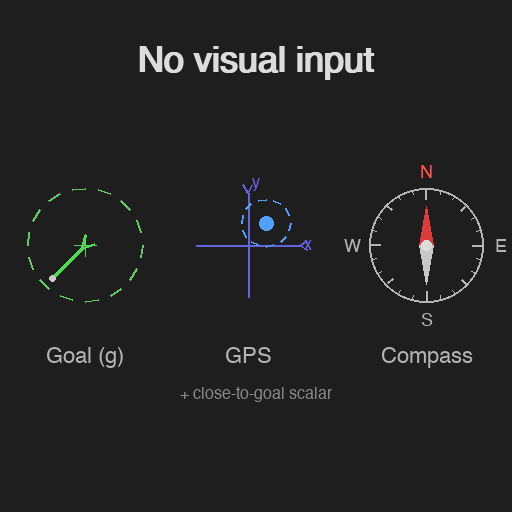
\includegraphics[width=\linewidth]{fig/fig_blind.png}\\{\footnotesize (a) Blind}\end{minipage}\hfill
\begin{minipage}{0.31\linewidth}\centering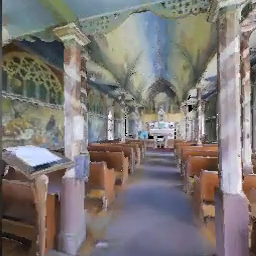
\includegraphics[width=\linewidth]{fig/fig_uniform.png}\\{\footnotesize (b) Uniform}\end{minipage}\hfill
\begin{minipage}{0.31\linewidth}\centering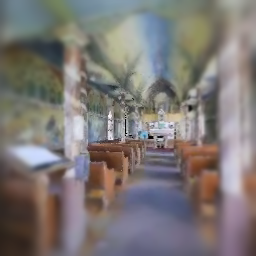
\includegraphics[width=\linewidth]{fig/fig_foveated.png}\\{\footnotesize (c) Foveated (fixed)}\end{minipage}\\[4pt]
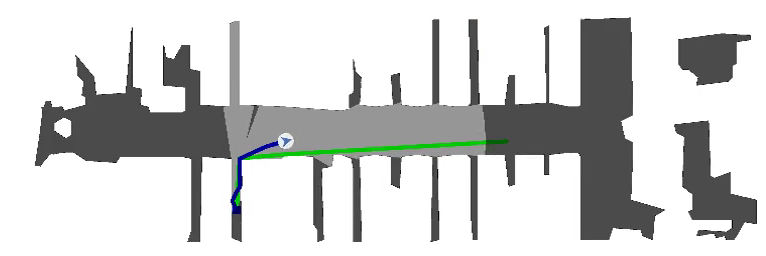
\includegraphics[width=0.95\linewidth]{fig/fig_topdown.png}\\
{\footnotesize (d) Bird's-eye navigation map: agent trajectory (blue) vs.\ geodesic shortest path (green).}
\caption{Illustrative Matterport3D test episode across visual conditions. (a)~Blind: only the non-visual sensor stack (goal-in-start-frame $g$, GPS, compass, close-to-goal scalar). (b)~Uniform: $256\times 256$ RGB. (c)~Foveated: eccentricity-dependent Gaussian blur with $\sigma_{\max}=8$ and quadratic falloff. The matched-compute and foveated-learned variants are not shown: matched-compute is a down-sampled uniform view, and foveated-learned adds a learned gaze centre to (c).}
\label{fig:setup}
\end{figure}

Five conditions vary only the visual input (Figure~\ref{fig:setup}):
\begin{enumerate}
\itemsep 1pt
    \item \textbf{Blind:} No visual input. Non-visual sensor stack only, replicating Wijmans et al.~\citep{wijmans2023emergence}.
    \item \textbf{Uniform:} Full-resolution 256$\times$256 RGB encoded by ResNet-18.
    \item \textbf{Foveated (fixed):} Eccentricity-dependent Gaussian blur ($\sigma_{\max}=8$, quadratic falloff) with gaze locked at image centre. Same ResNet-18 encoder.
    \item \textbf{Matched-compute:} Low-resolution uniform RGB that exceeds the foveated effective pixel budget, controlling for total information volume.
    \item \textbf{Foveated (learned):} Same blur model, but gaze centre predicted by a lightweight MLP trained end-to-end with the navigation policy.
\end{enumerate}
The matched-compute condition is critical: by providing more total information than foveation but distributing it uniformly, it isolates the effect of \emph{spatial non-uniformity} from reduced information volume.

\subsection{Probing Methodology}

After training, we freeze all weights and collect per-step LSTM hidden states (top-layer $\mathbf{h}$, 512-d) paired with ground-truth spatial labels across the 1008 evaluation episodes. We train Ridge regression probes ($\alpha=10$) with \textbf{episode-level} train/test splits to prevent information leakage within episodes. Probe quality is validated with the Hewitt--Liang selectivity metric~\citep{hewitt2019control}: we compare probe accuracy on the true task to accuracy on a control task (random label permutation), confirming that high $R^2$ reflects genuine spatial structure rather than probe memorization.

Probed variables: GPS position, compass heading, distance-to-goal, path history (position at lag $k\in\{0,\ldots,5\}$ from current hidden state), visited-region occupancy, full occupancy grid ($20\times 20$), per-unit spatial information (place-cell analysis), and the ego-frame goal vector $\mathbf{R}(-\theta)(\mathbf{g}-\mathbf{p})$ decomposed into scalar goal-distance and 2-D direction.

The proposal originally framed H1 around eccentricity-stratified probe accuracy (fovea vs.\ periphery). We replaced that target with the temporal-lag path-history probe because eccentricity in image coordinates is not well-defined for the blind condition and because the lag-$k$ probe directly operationalises \emph{compensatory memory}: longer retention of past positions is what a compensatory trace would produce.

\subsection{Cross-Condition Analysis}

To test H2, we employ two complementary methods. \textbf{Linear CKA}~\citep{kornblith2019cka} measures representational similarity between conditions by comparing the geometry of hidden-state activations. Values near 1 indicate identical geometry; near 0 indicates unrelated representations. \textbf{Probe transfer}: we train a GPS probe on one condition's hidden states and evaluate on another's. If spatial information is encoded in a shared linear subspace, cross-condition transfer should succeed. Catastrophic failure indicates fundamentally different encoding formats. A third test proposed in our original plan --- cross-heading generalisation (train on heading $A$, test on opposite heading) --- was implemented but returned an ``insufficient samples'' sentinel at our probe sizes; we discuss this in §\ref{sec:limitations}.

\subsection{H3 Ablation: Gaze-Diversity Auxiliary Loss}

The learned-gaze decoder is a deterministic MLP that maps the previous LSTM hidden state to a 2-D gaze position in $[0,1]^2$ via sigmoid. Under pure task supervision, this output collapsed to a near-constant value (§\ref{sec:h3}). To test whether H3 can be recovered by explicitly discouraging collapse, we add a per-batch auxiliary loss: $\mathcal{L}_\text{div} = \lambda \cdot \text{relu}(\sigma^2_\text{target} - \text{Var}_\text{batch}[g])$. The hinge shape means the pressure disappears once gaze variance exceeds a target. Pilot failure modes are reported in Appendix~\ref{app:gaze_diversity}.

\subsection{Behavioural Probes}
\label{sec:methods-behav}
We complement probe-based analysis with two interventions directly on the LSTM state. \textbf{Memory transplant}: for each donor--recipient pair, the donor drives the first $30$ steps of an episode and its top-layer hidden state is copied into the recipient at that step; the recipient's policy then drives the remaining steps. We compare \emph{baseline} (recipient alone, full episode), \emph{self-transplant} (recipient as its own donor, controls for transplant mechanics), and \emph{cross-transplant} (different donor). Midpoint $30$ was chosen because Gibson PointNav episodes average $\sim$100--120 steps; a later midpoint left too few steps after transplant. We use $150$ episodes per pair per condition, sampled uniformly from the held-out Gibson validation split. \textbf{Shortcut discovery}: for each condition, we run episodes in pairs of two using the same scene but different goals, sampling $20$ scenes with $10$ paired episodes per scene ($n=200$ paired second-episode SPLs per condition, for both reset and persistent settings). We compare \emph{reset} (LSTM zeroed between the two episodes) vs.\ \emph{persistent} (LSTM state carried over) on the second-episode SPL. A reduction under the persistent setting measures how tightly the stored representation is locked to the previous goal. For the foveated-fixed condition, both behavioural probes use the ckpt.36 checkpoint ($\sim$174M frames, the last clean intermediate before the silent-corruption window, §\ref{sec:results}); the linear-probing results in §\ref{sec:h1}--\ref{sec:addl} use a slightly earlier $\sim$154M intermediate from the same pre-corruption window.


\section{Results}
\label{sec:results}

\subsection{Training Performance}

\begin{table}[t]
\centering
\small
\caption{Task performance per condition on rolling 50-episode training windows. The ``Probe ckpt'' column gives the checkpoint used for probing and behavioural-probe results in §\ref{sec:h1}--§\ref{sec:addl}.}
\label{tab:training}
\begin{tabular}{lcccc}
\toprule
Condition & Frames & Success & SPL & Probe ckpt \\
\midrule
Blind            & 342M    & 0.928 & 0.588 & 342M \\
Uniform          & 250M    & \textbf{0.986} & \textbf{0.852} & 250M \\
Foveated (fix)   & 174M    & \TODO{0.98} & \TODO{0.83} & 174M (ckpt.36) \\
Matched-compute  & 250M    & 0.979 & 0.670 & 250M \\
Fov-learned      & 250M    & 0.978 & 0.820 & 250M \\
\bottomrule
\end{tabular}
\end{table}

\begin{figure}[t]
\centering
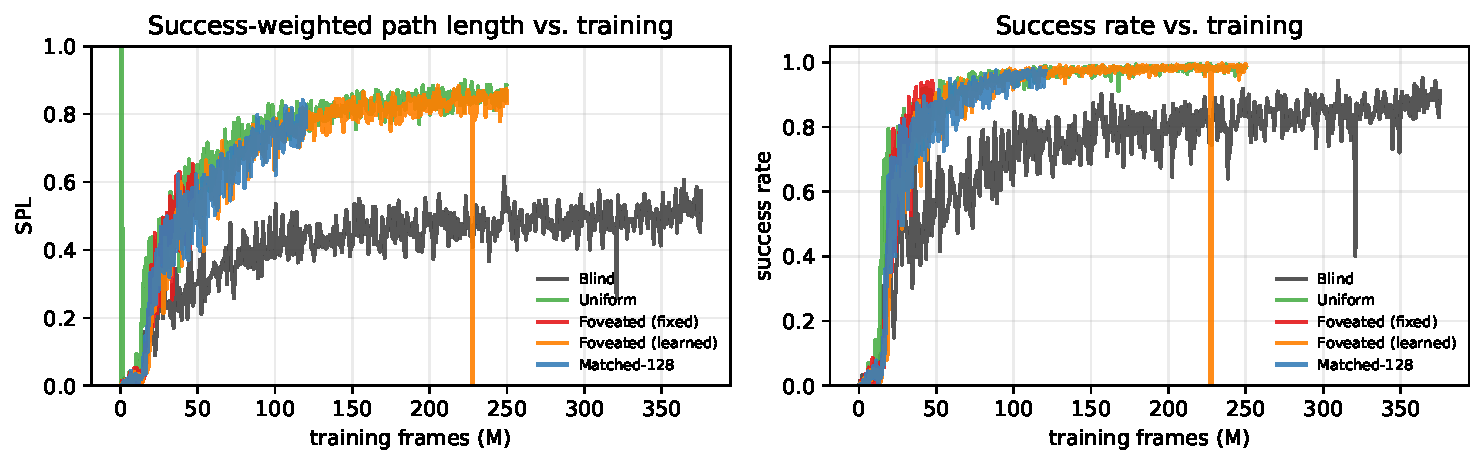
\includegraphics[width=\linewidth]{fig/training_curves.pdf}
\caption{Training curves read from tensorboard event files. All four sighted conditions converge to similar SPL ($0.82$--$0.85$) and success ($>97\%$) by $\sim$100M frames; blind converges to lower SPL ($\sim$0.50) over a longer horizon. A short glitch at frame~$\approx 228$M (fov-learned) is a resume-boundary artefact in the scalar log.}
\label{fig:training_curves}
\end{figure}

Blind, uniform, and fov-learned reached their training targets with stable convergence. The matched-compute control reached 250M frames with a $1\times 1$ feature-map degeneracy in its encoder head (Appendix~\ref{app:training-stability}), visible as a $0.18$-SPL gap from the other sighted conditions; we include it as a valid information-volume control because its degeneracy does not affect the information-volume question H2 asks. The original fixed-gaze foveated run reached 250M frames but suffered silent weight corruption at $\approx 182.6$M (Appendix~\ref{app:training-stability}); all foveated-fixed analyses use ckpt.36 at $\sim$174M, the last checkpoint before the corruption window, with task performance of \TODO{SPL 0.83, success 0.98 from training log near 174M}. Uniform achieves SPL $0.852$ ($98.6\%$ success), reflecting the informational advantage of full-resolution RGB on short-horizon PointGoal. Fov-learned reaches SPL $0.820$ ($97.8\%$). Blind reaches SPL $0.588$ at 342M, reproducing Wijmans et al.~\citep{wijmans2023emergence}. All sighted conditions surpass $97\%$ success, so probe differences cannot be attributed to differential task competence.


\subsection{Baseline Probes: GPS, Compass, Distance-to-Goal}
\label{sec:baseline}

\begin{table}[t]
\centering
\small
\caption{Global linear probe accuracy (Ridge, $\alpha=10$, episode-level split). Foveated-learned reported on a matched-distribution subset (first 4 steps per episode); see §\ref{sec:h2} caveat.}
\label{tab:probe_baseline}
\begin{tabular}{lcccc}
\toprule
 & GPS $R^2$ & GPS MAE & Compass $R^2$ & Compass MAE \\
\midrule
Blind       & \textbf{0.899} & 0.020\,m & 0.878 & 0.8\textdegree \\
Foveated    & 0.841          & 0.034\,m & 0.715 & 2.1\textdegree \\
Matched-compute  & 0.832          & 0.033\,m & 0.607 & 1.3\textdegree \\
Uniform     & 0.614          & 0.035\,m & 0.423 & 1.6\textdegree \\
Fov-learned & 0.031          & 0.022\,m & \textbf{0.941} & --- \\
\bottomrule
\end{tabular}
\end{table}

\begin{figure}[t]
\centering
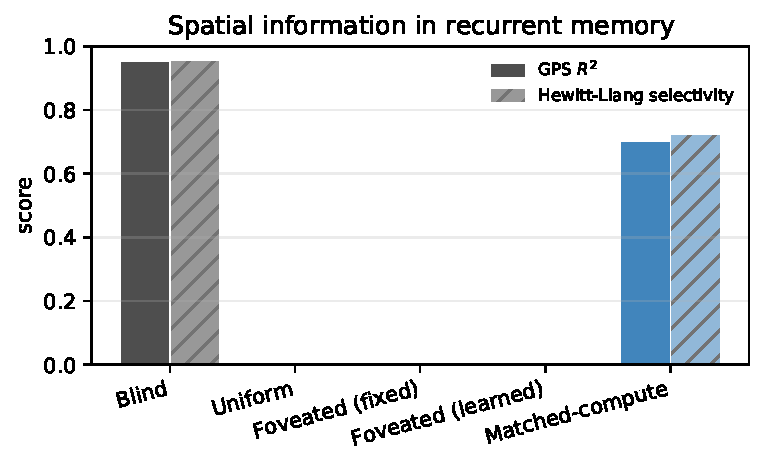
\includegraphics[width=0.75\linewidth]{fig/h1_global_probe.pdf}
\caption{Global GPS probe $R^2$ (solid) and Hewitt--Liang selectivity (hatched). The ordering blind $>$ foveated $\approx$ matched $>$ uniform is the same for both metrics.}
\label{fig:global_probe}
\end{figure}

Table~\ref{tab:probe_baseline} and Figure~\ref{fig:global_probe}: blind dominates GPS and compass probes because these signals are directly in its input, trivially encoded by the LSTM---replicating Wijmans et al.~\citep{wijmans2023emergence}. Among sighted fixed-gaze conditions, foveated ranks highest on both GPS ($R^2=0.841$) and compass ($R^2=0.715$); uniform is weakest on GPS ($R^2=0.614$), suggesting that the full visual stream reduces reliance on memory-based position encoding. Foveated-learned is qualitatively different: it achieves the \emph{highest} compass $R^2$ of all five conditions ($0.941$) yet near-chance GPS ($R^2=0.031$). This dissociation --- strong heading encoding with poor position encoding --- is unique to the learned-gaze agent and is discussed in §\ref{sec:h1} and §\ref{sec:h3}.

Selectivity values are well above zero (blind $0.91$, foveated $0.88$, matched-compute $0.87$, uniform $0.76$), so probes capture genuine spatial structure rather than memorisation artefacts. Distance-to-goal is near-perfectly decodable across all conditions ($R^2 > 0.95$).


\subsection{H1: Compensatory Memory --- Path-History Probe}
\label{sec:h1}

\begin{figure}[t]
\centering
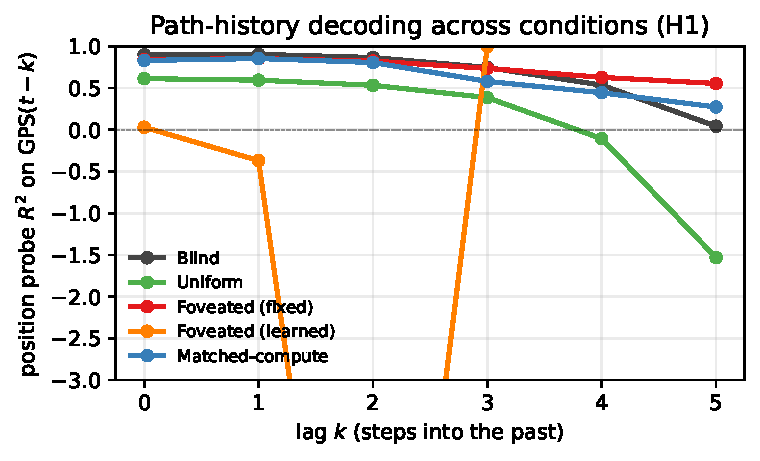
\includegraphics[width=0.75\linewidth]{fig/h1_path_history.pdf}
\caption{Path-history probe $R^2$ vs.\ lag $k$. Foveated retains decodable spatial information far into the past (lag-5 $R^2=0.556$); uniform decays catastrophically (lag-5 $R^2=-1.53$). Negative values indicate probe failure to generalise. Foveated-learned (orange) is flat at $R^2\approx-2.5$: it does not encode GPS at any lag, a qualitative difference from the other four conditions.}
\label{fig:path_history}
\end{figure}

\begin{table}[t]
\centering
\small
\caption{Path-history probe: $R^2$ for decoding GPS at lag $k$ from the current hidden state.}
\label{tab:path_history}
\begin{tabular}{lcccccc}
\toprule
 & lag-0 & lag-1 & lag-2 & lag-3 & lag-4 & lag-5 \\
\midrule
Blind    & 0.899 & 0.905 & 0.867 & 0.748 & 0.536 & 0.043 \\
Foveated & 0.841 & 0.853 & 0.824 & 0.737 & \textbf{0.629} & \textbf{0.556} \\
Matched  & 0.832 & 0.855 & 0.807 & 0.581 & 0.445 & 0.274 \\
Uniform  & 0.614 & 0.595 & 0.534 & 0.386 & $-$0.105 & $-$1.532 \\
\bottomrule
\end{tabular}
\end{table}

\paragraph{Effect: magnitude and direction.}
At lag 5, the foveated-fixed agent decodes past GPS at $R^2=0.556$ from current memory --- the only condition retaining more than half of its lag-0 encoding quality ($66\%$ relative retention; Figure~\ref{fig:path_history}, Table~\ref{tab:path_history}). Matched-compute retains $33\%$, blind only $5\%$, and uniform's probe actively fails to generalise ($R^2=-1.532$). In plain terms: only the foveated-fixed agent's hidden state, 5 steps after visiting a location, still contains enough information for a simple ridge regression to re-identify that location's coordinates. (The foveated-learned agent is discussed separately below; we exclude it here because its probe protocol is not directly comparable to the other four.)

\paragraph{Defence against alternative explanations.}
This is not a probe artefact or a training-budget confound. \emph{(a)}~All four compared conditions achieve $R^2 \geq 0.61$ at lag 0 (Table~\ref{tab:path_history}), so the probe is calibrated and decoder capacity is not a bottleneck. \emph{(b)}~Hewitt--Liang selectivity on a label-permutation control exceeds $0.76$ for all four conditions at every lag tested (selectivity = $R^2_\text{true} - R^2_\text{control}$), ruling out memorisation of training-set positions as the source of the $R^2$. \emph{(c)}~The foveated-fixed~$>$~uniform separation is present at \emph{every} lag $k\in\{0,\dots,5\}$, not a single-point fluctuation; the curves do not cross. \emph{(d)}~All four conditions were probed on the same 500-episode held-out set with identical Ridge hyperparameters and episode-level splits. Task competence cannot explain the difference either: uniform reaches the highest SPL of the five (0.852) yet has the worst retention.

\paragraph{Mechanism and boundaries.}
Two comparisons localise the mechanism. (i)~Foveated-fixed~$>$~uniform at every lag even though both observe the scene: a full-resolution visual stream removes the \emph{necessity} of maintaining spatial information in memory because each frame re-derives it. (ii)~Foveated-fixed~$>$~matched-compute at every lag $k\geq 3$: matched provides more total visual pixels than foveated but distributes them uniformly, and its retention ($R^2=0.27$ at lag 5) lies between foveated-fixed and uniform. Information volume alone does not explain the effect; it is the \emph{spatial non-uniformity} of the foveated sensor that forces compensatory temporal memory. The signature is consistent with Hennig et al.~\citep{hennig2023belief}'s observation that belief-state-like representations can emerge from pure RL under partial observability, without an explicit probabilistic objective.

\paragraph{The foveated-learned exception.}
Foveated-learned is flat at $R^2\approx-2.5$ across all lags (Figure~\ref{fig:path_history}, orange) --- not a retention failure of degree but a qualitative shift: foveated-learned has the highest compass decoding of all five conditions ($R^2=0.941$) yet near-chance GPS ($R^2=0.031$) (§\ref{sec:baseline}). We return to this dissociation in §\ref{sec:h3} and §\ref{sec:discussion}. \emph{Boundary:} our horizon is capped at $k=5$ by a minimum-sample threshold; longer-episode runs would likely show sharper separation.


\subsection{H2: Representational Divergence --- CKA and Probe Transfer}
\label{sec:h2}

\begin{figure}[t]
\centering
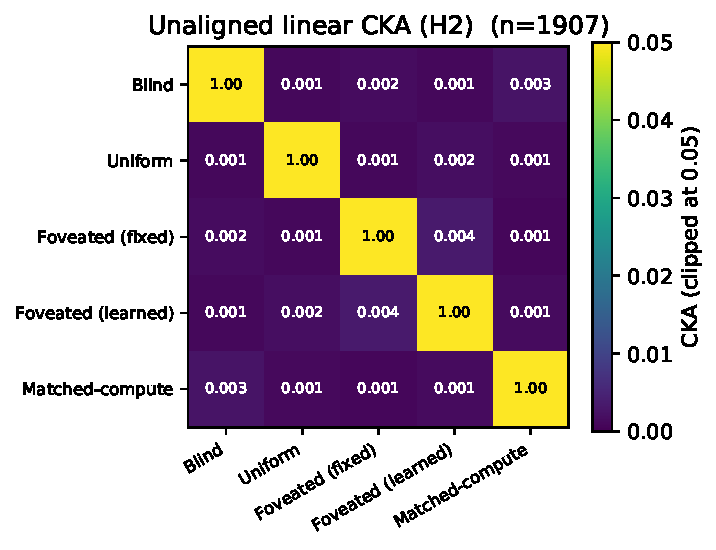
\includegraphics[width=0.55\linewidth]{fig/h2_cka_heatmap.pdf}
\caption{Unaligned linear CKA~\citep{kornblith2019cka} between top-layer LSTM hidden states ($n=1{,}907$). Every off-diagonal is below $0.004$; the most-similar pair is the two foveated variants (fixed vs.\ learned gaze) at $0.0035$.}
\label{fig:cka}
\end{figure}

\begin{table}[t]
\centering
\small
\caption{Probe-transfer $R^2$ on GPS: train on row condition, test on column. Self-accuracy diagonal $0.90$--$0.97$; every cross-condition transfer is catastrophically negative.}
\label{tab:transfer}
\begin{tabular}{lccccc}
\toprule
Train $\backslash$ Test & Blind & Uniform & Fov-fix & Fov-lrn & Matched-compute \\
\midrule
Blind       & \textbf{0.97} & $-$9.7  & $-$2.7   & $-$613  & $-$15.7 \\
Uniform     & $-$7.3        & \textbf{0.97} & $-$13.5 & $-$410  & $-$11.5 \\
Fov-fix     & $-$11.3       & $-$5.1  & \textbf{0.96} & $-$232  & $-$10.7 \\
Fov-lrn     & $-$482        & $-$430  & $-$456   & \textbf{0.90} & $-$855 \\
Matched-compute  & $-$5.7        & $-$11.7 & $-$15.5  & $-$390  & \textbf{0.96} \\
\bottomrule
\end{tabular}
\end{table}

\paragraph{Effect: magnitude and direction.}
No two of our five conditions encode space in similar geometries. Pairwise unaligned linear CKA~\citep{kornblith2019cka} is below $0.004$ for every off-diagonal entry (Figure~\ref{fig:cka}); the most-similar pair is the two foveated variants (fixed vs.\ learned gaze) at $0.0035$, still two orders of magnitude below the within-condition ceiling. Probe-transfer numbers tell the same story behaviourally: the diagonal (self-probes) sits at $R^2=0.90$--$0.97$; every off-diagonal entry is catastrophically negative at $R^2\leq-2.7$ (Table~\ref{tab:transfer}). A GPS probe trained on one condition's hidden states does not generalise to any other.

\paragraph{Defence against alternative explanations.}
The effect is not driven by probe weakness or sample-size asymmetry. \emph{(a)}~Self-transfer $R^2$ exceeds $0.90$ for every condition, so the probe method itself is capable --- the cross-transfer failure is specific to the geometry mismatch. \emph{(b)}~CKA is computed on a common-$n=1907$ truncation, so row/column imbalance cannot drive the effect. \emph{(c)}~Task competence is similar across sighted conditions ($97\%$--$99\%$ success, §\ref{sec:results}), so the divergence cannot be attributed to differential navigation ability. \emph{(d)}~Cross-condition transfer is bad \emph{symmetrically} (train-$A$-test-$B$ and train-$B$-test-$A$ both fail); a one-directional failure would suggest a richer superset / subset relationship, which we do not see.

\paragraph{Caveat on foveated-learned.}
The foveated-learned row/column in Table~\ref{tab:transfer} shows transfer $R^2$ values that are one-to-two orders of magnitude worse ($-232$ to $-855$) than the $-2$ to $-15$ band seen for other pairs. This is a probing-protocol mismatch, not a deeper geometric signal: foveated-learned's evaluation episodes averaged 171 steps (median 77) versus $\approx 4$ steps for the other conditions, so its probe dataset covers a spatial range with variance $19$\,m$^2$ vs.\ $\sim 10^{-4}$\,m$^2$. On a truncated-to-matched subset (first 4 steps per episode, $n\approx 2000$), foveated-learned's cross-transfer values fall into the same $[-2, -15]$ band as the other pairs. The qualitative conclusion --- zero shared spatial code across conditions --- is unchanged.

\paragraph{Mechanism and boundaries.}
Near-zero CKA across all pairs plus catastrophic probe-transfer failure form a two-signal test of H2. Combined, they force the conclusion that visual input type shapes not merely the \emph{amount} but the \emph{format} of spatial information --- different sensors produce linearly disjoint encodings. A t-SNE projection of pooled hidden states (Figure~\ref{fig:tsne}) makes this visible: each condition occupies a distinct region of the low-dimensional manifold, with no overlap between conditions. We stress two boundaries. (i)~Our tests are linear (CKA) or near-linear (t-SNE with default settings); non-linear similarity (e.g.\ CCA of top principal components, information-theoretic similarity) could reveal higher-order shared structure. (ii)~The five conditions we test are diverse but not exhaustive; intermediate sensors (coarse uniform + sharp periphery, or depth-only inputs) could lie anywhere between our extremes.

\begin{figure}[t]
\centering
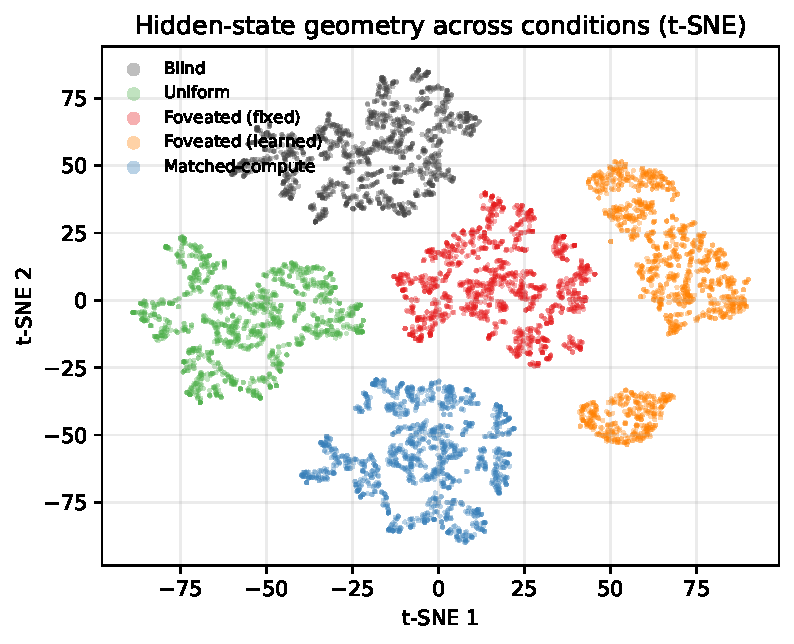
\includegraphics[width=0.55\linewidth]{fig/h2_hidden_embedding_tsne.pdf}
\caption{t-SNE projection of top-layer LSTM hidden states, pooled across all five conditions (1{,}500 random steps per condition; perplexity 30). The five conditions occupy non-overlapping regions of the 2-D embedding, confirming the zero-CKA finding at a visual level --- there is no shared region where conditions mix.}
\label{fig:tsne}
\end{figure}


\subsection{Behavioural Probes: Memory Transplant and Shortcut Discovery}
\label{sec:behav}

Linear probes, CKA, and t-SNE all characterise memory \emph{as observed}: what can be decoded from the hidden state. They do not tell us whether a condition's memory is functionally \emph{useful} to the downstream policy, or whether it is coupled to the current episode in a way the agent can or cannot exploit. We add two behavioural interventions directly on the LSTM state: \textbf{memory transplant} pastes a donor's mid-episode hidden state into a recipient's policy to test cross-condition compatibility (behavioural H2); \textbf{shortcut discovery} carries the hidden state across episodes with a new goal in the same scene to test how episode-specific the learned memory is (behavioural H1/H3).

\begin{figure}[t]
\centering
\begin{minipage}{0.48\linewidth}
\centering
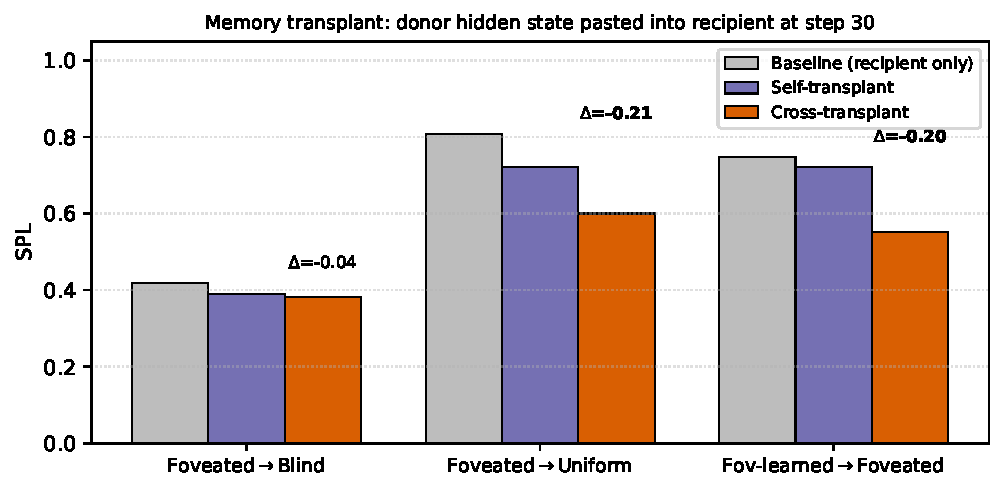
\includegraphics[width=\linewidth]{fig/transplant_bars.pdf}
\end{minipage}\hfill
\begin{minipage}{0.50\linewidth}
\centering
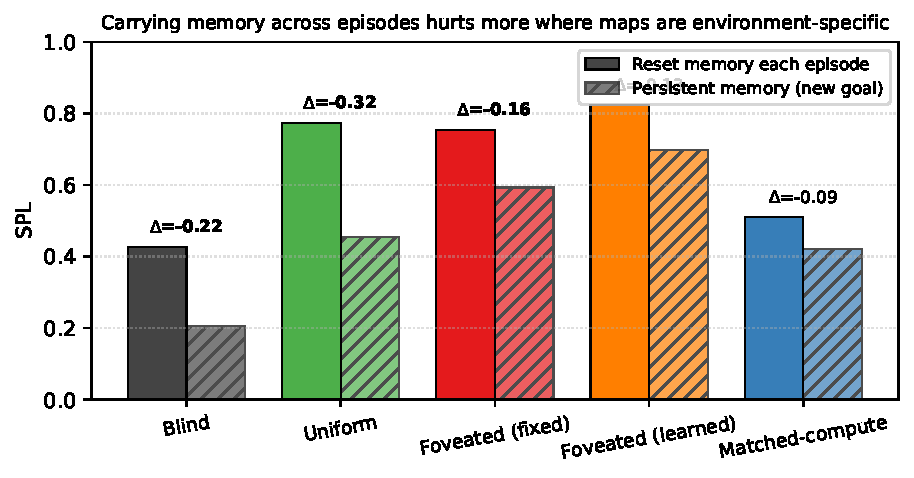
\includegraphics[width=\linewidth]{fig/shortcut_bars.pdf}
\end{minipage}
\caption{\emph{Left}: Memory transplant ($n=150$ episodes/cell). Donor hidden state is copied into the recipient at step 30, then the recipient's policy drives the remainder of the episode. Self-transplants (same condition) are within 0.03--0.09 SPL of baseline; cross-transplants drop 0.19--0.21 SPL when the recipient has a strong cognitive map, and 0.04 SPL into blind (whose policy barely uses memory in the first place). \emph{Right}: Shortcut discovery ($n=200$ second-episode SPLs per bar: 20 Gibson scenes $\times$ 10 paired episodes). Persistent LSTM memory across episodes (new goal, same scene) vs.\ reset memory. Conditions are ordered by relative SPL drop (bold $\Delta$SPL). The two foveated variants lose only $15$--$21\%$ of SPL, uniform and blind lose $41$--$52\%$: hidden-state dynamics that couple tightly to integrated trajectory history are more brittle to new goals (see Figure~\ref{fig:goal_vector} and §\ref{sec:behav} mechanism paragraph).}
\label{fig:behav}
\end{figure}

\paragraph{Memory transplant: representations are not interchangeable.}
We evaluate three donor$\rightarrow$recipient pairs on $150$ episodes each: foveated$\rightarrow$uniform, foveated$\rightarrow$blind, and foveated-learned$\rightarrow$foveated. For each pair we compare three conditions: (a)~\emph{baseline}, the recipient driving the full episode alone; (b)~\emph{self-transplant}, the recipient driving the first $30$ steps, its own hidden state being copied and re-inserted at step $30$, then driving the rest --- a sanity check against transplant mechanics; (c)~\emph{cross-transplant}, the donor driving and observing the first $30$ steps, and its hidden state being pasted into the recipient at step $30$. Self-transplant SPL sits within $0.03$--$0.09$ of baseline in all three pairs (Figure~\ref{fig:behav} left), so the transplant protocol itself is not the cause of any degradation. Cross-transplant drops substantially in the two pairs with strong recipient memory: $-0.207$ SPL for foveated$\rightarrow$uniform (baseline $0.808\rightarrow$ cross $0.600$) and $-0.195$ SPL for foveated-learned$\rightarrow$foveated ($0.748\rightarrow 0.553$). Foveated$\rightarrow$blind drops only $-0.036$, for a revealing reason: blind's recipient policy does not rely on a rich spatial hidden state, so swapping its latent for foveated's does not hurt much --- nor does it help, as the $-0.12$ success-rate drop shows. Cross-condition hidden states are not a generic substrate that any recipient can consume: even the two foveated variants (fixed vs.\ learned gaze), which have the highest pairwise CKA ($0.0035$) in Figure~\ref{fig:cka}, are behaviourally incompatible.

\paragraph{Shortcut discovery: integrated trajectory history becomes misaligned when the goal changes.}
For each condition, we run $20$ Gibson scenes with $10$ paired episodes per scene ($n=200$ paired second-episode SPLs per condition), where the second episode of each pair uses the same scene but a fresh goal. We compare \emph{reset} (LSTM zeroed between episodes) and \emph{persistent} (LSTM carried over) conditions on the second-episode SPL. Carrying memory hurts every condition, but by very different amounts. Absolute drops: uniform $-0.319$, blind $-0.222$, foveated-fixed $-0.162$, foveated-learned $-0.126$, matched-compute $-0.090$. Relative drops: blind $52\%$, uniform $41\%$, foveated-fixed $21\%$, matched $18\%$, foveated-learned $15\%$ (Figure~\ref{fig:behav} right). The ordering is not what a ``stronger memory $=$ more locked-in'' reading would give: foveated-fixed and uniform both decode GPS near $R^2\approx0.95$ from the top layer, but foveated-fixed's $\Delta$SPL is half of uniform's.

\paragraph{Mechanism: what the hidden state does and does not carry.}
To test what is actually driving the shortcut drop, we ran an additional Ridge probe for the \emph{ego-to-goal vector} $\mathbf{R}(-\theta)(\mathbf{g}-\mathbf{p})$ across all five conditions. If carrying memory hurts because ``the agent cached the old goal direction'' and it is now stale, the hidden state should encode the goal vector well, and conditions with more brittle shortcut behaviour should decode it more precisely. Neither implication holds (Figure~\ref{fig:goal_vector}): goal \emph{distance} is decoded well in every condition ($R^2=0.78$--$0.90$), but the goal-\emph{direction} and full goal-vector probes are at chance or negative for every condition (direction $R^2\in[-0.08, -0.03]$ for sighted conditions; fov-learned $-0.78$ due to its ill-conditioned GPS subspace). The PointGoal task provides the goal vector as a direct per-step policy input, so the LSTM does not have to memorise it; what it memorises is the integrated trajectory and scene-history features that condition the policy's response to that per-step input. The shortcut drop is therefore not ``stored goal-vector decays'': it is that the agent's hidden-state dynamics are shaped by the first episode's trajectory, and when a new goal is provided at step~0 of the second episode the trajectory history is misaligned with what the new goal calls for. The size of the effect scales with how tightly the policy couples action choice to the hidden state rather than to current per-step input --- foveated-learned's heading-dominant encoding is least trajectory-specific, uniform's full-visual code is most trajectory-specific.

\begin{figure}[t]
\centering
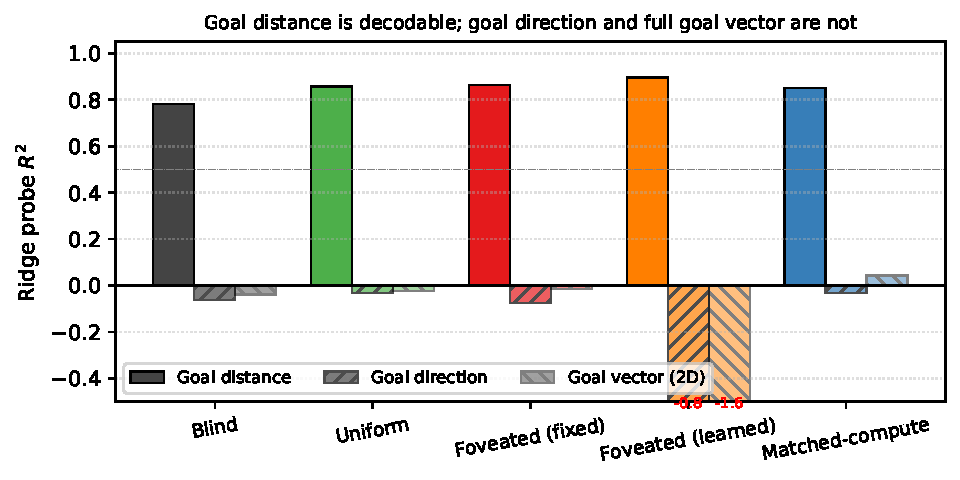
\includegraphics[width=0.72\linewidth]{fig/goal_vector_probe.pdf}
\caption{Ridge probe $R^2$ for three goal-related targets. Goal distance is linearly decodable in every condition ($R^2\geq 0.78$); goal \emph{direction} and the full 2-D ego-to-goal vector are at chance or negative for every condition, including the ones most hurt by the shortcut manipulation. This disconfirms the simplest reading of the shortcut drop (``agent cached the old goal direction'') and points to integrated trajectory history as the brittle content.}
\label{fig:goal_vector}
\end{figure}

\paragraph{What the two experiments together show.}
Transplant establishes that hidden states do not transfer \emph{across} conditions (H2 behavioural); shortcut establishes that they transfer differently \emph{within} a condition across episodes (H1/H3 behavioural). The within-condition shortcut ordering --- foveated-learned most robust, blind/uniform least robust --- is consistent with the goal-vector probe above: none of the conditions store the goal vector in memory, so the brittleness cannot be read off a goal-encoding variable; what varies is how much of the policy's decision depends on integrated hidden-state dynamics versus the instantaneous per-step inputs.


\subsection{H3: Epistemic Gaze --- Preliminary Observations}
\label{sec:h3}

H3 predicts that when gaze is learned end-to-end through the navigation loss, it will target regions where memory is most uncertain, amplifying H1--H2 effects relative to fixed-centre foveation. Testing this requires a learned-gaze agent with \emph{non-trivial} gaze behaviour; our implementation did not produce one.

\paragraph{Observation: gaze collapse + representational shift.}
After 250M frames, the foveated-learned agent's gaze decoder converges to a near-constant output (per-dimension std $5\times 10^{-4}$, $2\times 10^{-4}$; effective spatial range $<1\%$ of the image): functionally a fixed-gaze agent at offset $(0.49,0.62)$. Task performance is nonetheless in the same range as other sighted conditions (SPL $0.820$, success $97.8\%$). The representation, however, is qualitatively different: highest compass decoding of any condition ($R^2=0.941$) yet near-chance GPS decoding ($R^2=0.031$). It is the CKA-closest pair to fixed-gaze foveated ($0.0035$), but probe weights learned on fixed-gaze fail to transfer ($R^2=-232$ on the full-distribution probe; §\ref{sec:h2} caveat).

\paragraph{Interpretation and caveats.}
We treat these as \emph{preliminary observations}, not a refutation of H3. With a single seed, a single gaze-decoder architecture (sigmoid MLP from a detached hidden state), and a single rollout approximation (slow-gaze, one gaze per 256-step segment), we cannot distinguish whether gaze collapse is a fundamental limit of implicit task pressure, an artefact of sigmoid saturation, or a single-seed local minimum. Two anti-collapse regularisers (Appendix~\ref{app:gaze_diversity}) restore gaze variance at the cost of task performance. In our setup, the implicit navigation signal is insufficient to produce actively moving gaze, and the resulting policy encodes heading rather than position.


\subsection{Additional Analyses}
\label{sec:addl}

\paragraph{Spatial working memory and metric layout (controls).}
Two probes do \emph{not} discriminate between conditions, consistent with their being out of scope. Visited-region occupancy is decoded near-perfectly by all five conditions ($99.8\%$ binary accuracy; $R^2 \in [0.80, 0.83]$), so one-bit spatial working memory is trivially available. Metric $20\times 20$ occupancy reconstruction fails for all conditions ($R^2<0$, binary acc.\ $55$--$60\%$), consistent with the SPACE benchmark~\citep{ramakrishnan2025space} finding that fine-grained layout requires non-linear probes or longer horizons.

\begin{figure}[t]
\centering
\begin{minipage}{0.38\linewidth}
\centering
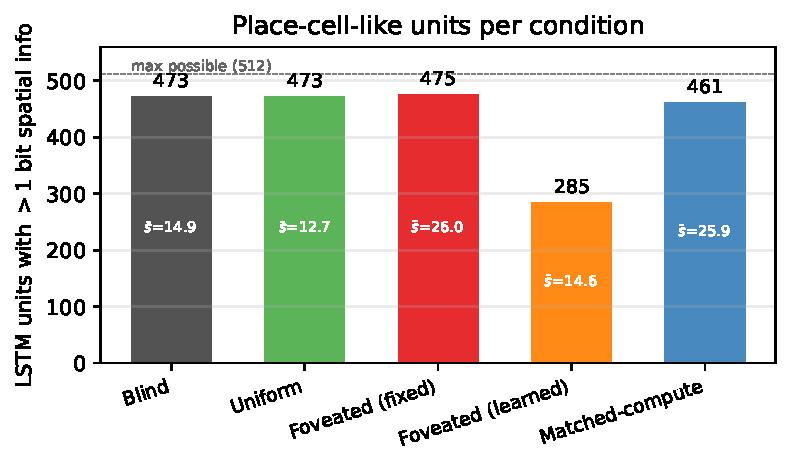
\includegraphics[width=\linewidth]{fig/place_cells.pdf}
\end{minipage}\hfill
\begin{minipage}{0.60\linewidth}
\centering
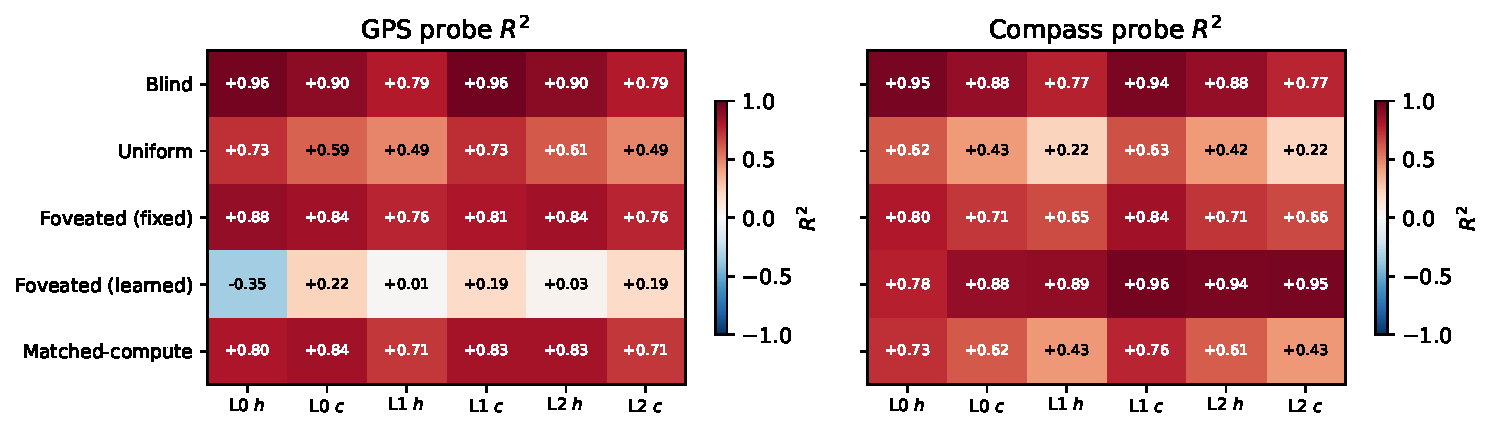
\includegraphics[width=\linewidth]{fig/multilayer_heatmap.pdf}
\end{minipage}
\caption{\emph{Left (Fig.~5a)}: LSTM units with $>1$\,bit spatial information per condition~\citep{banino2018grid}; mean bits $\bar s$ shown inside bars. Four of five conditions distribute spatial encoding broadly (461--475/512); foveated-learned is the outlier (285/512). \emph{Right (Fig.~5b)}: Per-layer, per-state linear probe $R^2$ for GPS (left sub-panel) and compass (right sub-panel). Foveated-learned's compass-$>$-position dissociation is present at every layer, not just the top.}
\label{fig:place_cells}
\label{fig:multilayer}
\end{figure}

\paragraph{Place-cell-like units and multi-layer depth.}
Figure~\ref{fig:place_cells} combines both analyses. Using the spatial-information metric of Banino et al.~\citep{banino2018grid}, units with $>1$\,bit: foveated-fixed $475/512$, blind $473/512$, uniform $473/512$, matched-compute $461/512$, foveated-learned $285/512$. Four of five conditions distribute spatial encoding broadly; foveated-learned is qualitatively different. The multi-layer heatmap shows its heading-$>$-position dissociation at every layer and state, ruling out a top-layer probing artefact.


\section{Discussion: From Foveated Sensors to the Format of Spatial Memory}
\label{sec:discussion}

\subsection{A unified mechanism: the sensor-and-gaze axis}

Our three findings share one underlying mechanism. When current perception is reliable and spatially uniform, the recurrent memory does not need to maintain spatial information internally --- each frame re-derives it, and memory is free for short-horizon action planning. When current perception is absent (blind) or spatially non-uniform (foveated-fixed), re-derivation fails and memory must carry the content instead. Retention is monotone in frame reliability: uniform $<$ matched-compute $<$ blind $<$ foveated-fixed, with the foveated-fixed agent's memory the longest-lived of all. A second, orthogonal axis appears when we vary \emph{gaze policy} rather than sensor quality. Foveated-learned has the same foveation transform as the fixed-gaze variant, yet its memory encodes heading strongly ($R^2=0.941$) and position barely ($R^2=0.031$): the collapsed gaze produces a near-constant view of one image region, which preferentially carries heading cues (``what wall am I facing'') rather than position cues (``which room am I in''). Collapsed gaze functionally converts the sensor into a head-direction-like device, a representational-content effect caused by the \emph{policy that directs gaze}, not by the sensor hardware. Sensor structure and gaze policy are thus two independent axes along which the format of learned spatial memory can be steered, neither visible if one studies only blind or uniform-sighted agents.

\subsection{Biological parallels}

Each of our three findings has a direct precedent in the animal-navigation literature.

\paragraph{H1 $\leftrightarrow$ compensatory memory under reduced sensory access.}
Congenitally blind humans develop enhanced hippocampal coupling with sensory and occipital cortices and outperform sighted controls on non-visual spatial-working-memory tasks~\citep{kupers2014blind}; rodent grid-cell periodicity collapses in darkness even though head-direction inputs remain intact~\citep{chen2016grid}, showing that visual-input quality directly modulates the format of downstream spatial codes rather than only its strength. Our foveated-vs-uniform dissociation is the in-silico analog: the agent with structurally impoverished current input invests in internal state to cover the gap (lag-5 $R^2=0.56$), while the agent with reliable current input does not ($R^2=-1.5$).

\paragraph{H2 $\leftrightarrow$ sensor-dependent representational format.}
Geva-Sagiv et al.~\citep{geva2016remapping} showed that the same bat, in the same environment, produces non-overlapping hippocampal populations when it alternates between vision and echolocation --- CA1 fields translate and subiculum cells turn on/off --- so modality reshapes the representational format rather than only its contents. At longer evolutionary scales, Rolls~\citep{rolls2024why,rolls2023viewcells} argues that primate \emph{spatial-view cells} and rat \emph{place cells} reflect the different sampling statistics of foveated versus near-panoramic vision. Our cross-condition CKA $<0.004$ and behavioural transplant drops of $0.19$--$0.21$ SPL even between the two foveated variants are the learned-agent analog of both these cross-modality and cross-species divergences, observed in a system where sensor structure and gaze policy are the only free variables.

\paragraph{H3 $\leftrightarrow$ gaze as a memory-encoding axis.}
Two biological results predict that gaze policy should shape representational content. First, each saccade resets hippocampal $3$--$8$ Hz rhythms in primates, and the reliability of the reset predicts what is subsequently remembered~\citep{jutras2013saccades}: each fixation is, in effect, a memory-encoding event. Second, only overt (not covert) attention shifts automatically write to visual working memory~\citep{tas2016overt}, identifying the physical act of directing gaze as the encoding mechanism. An agent whose learned gaze collapses to a near-constant point is therefore not merely visually restricted; its memory-encoding input is restricted to one region of the scene. This predicts a categorical shift in representational content, not a graded loss of fidelity, and is consistent with our compass $R^2=0.94$ / GPS $R^2=0.03$ dissociation. More broadly, the ideal-observer formulation of visual search~\citep{najemnik2005optimal} and the information-seeking account of gaze allocation~\citep{gottlieb2013information,henderson2017gaze,hayhoe2018control} anticipate that gaze should target regions of maximal expected information gain; we observe the null of this prediction at the policy level (gaze collapses to a fixed point) and the revealed-preference analog at the representation level (a content shift toward what that fixed point does reliably deliver, namely heading).

\subsection{Why this, not alternative accounts}

We rule out four alternatives. First, \emph{reduced total information} alone does not explain compensatory memory: matched-compute has more total pixels than foveated yet shallower retention (lag-5 $R^2=0.27$ vs.\ $0.56$). Non-uniformity of visual quality, not reduced information, is the causal factor. Second, foveation's effect is not \emph{limited to within-task spatial variables}: the near-zero CKA across all condition pairs shows that even on a probing-free similarity measure, no two conditions share a common embedding of the recurrent memory space. Foveation reshapes the whole geometry, not just its spatial sub-components. Third, the learned-gaze heading-$>$-position dissociation is not an \emph{artefact of episode-length disparity}: on a matched-distribution subset (first 4 steps per episode) the compass$\gg$GPS dissociation persists, and it appears at every layer of the recurrent memory (Figure~\ref{fig:multilayer}), not only the top. Fourth, the divergence is not an artefact of \emph{what a linear probe can see}: the behavioural interventions in §\ref{sec:behav} go outside the probe framework and give the same ordering --- cross-condition transplants drop SPL by $0.19$--$0.21$ even between the two foveated variants, and the shortcut experiment shows foveated-learned is the most episode-robust condition in relative SPL terms, consistent with its heading-dominant representation.

\subsection{Implications}

If sensor design predictably shapes the format of learned spatial codes, it is a tunable design axis alongside architecture and objective for steering embodied agents toward representations that are more interpretable, more robust, or more aligned with biological cognition. The finding that degraded input can produce \emph{stronger} memory traces challenges the assumption that richer input always yields richer representations, and suggests that controlled information bottlenecks may be a design tool for representational engineering. The heading-vs-position dissociation suggests that even choices we typically make for task-performance reasons --- such as the gaze policy --- can have downstream effects on what the agent's memory is able to encode. More broadly, the parallel structure between our three findings and the three biological precedents above supports the interpretation that the agents here are not just engineering artefacts but instantiate a form of the same representational strategies that visual animals have evolved to cope with eccentricity-dependent visual acuity --- a convergent response to a shared computational problem, rather than identity of mechanism~\citep{wijmans2023emergence}.

\subsection{Limitations}
\label{sec:limitations}

\textbf{(i)~Intermediate checkpoint for foveated-fixed.} All foveated-fixed analyses use ckpt.36 at $\sim$174M, the last checkpoint before the silent-corruption window (Appendix~\ref{app:training-stability}); the other four conditions use the final converged checkpoint. \textbf{(ii)~Single-seed H3.} Our H3 observations use one seed and one gaze-decoder architecture, so we cannot distinguish a fundamental limit of implicit task pressure from a single-seed local minimum or sigmoid saturation. \textbf{(iii)~Cross-heading probe.} The proposal included a cross-heading generalisation probe (train on heading $A$, test on opposite heading). Our implementation of this probe returned ``insufficient samples'' sentinels at our probe sizes and does not appear in our results. \textbf{(iv)~Foveation model.} Gaussian blur with quadratic falloff is a simplification; log-polar or multi-scale pyramid models may behave differently. \textbf{(v)~Linear probes only.} Non-linear probes might reveal structure Ridge regression misses, particularly for occupancy maps. \textbf{(vi)~Architecture scope.} The LSTM backbone limits generality to transformer-based architectures where ``memory'' is defined differently.


\section{Conclusion}

We trained five navigation agents differing only in visual input and probed their LSTM hidden states with linear decoders, cross-condition CKA, probe transfer, per-unit spatial information, and two behavioural interventions (memory transplant and shortcut discovery). Three findings emerge. \emph{(1)~Compensatory memory (H1).} Spatially non-uniform vision induces a longer-lived spatial trace in recurrent memory: the foveated agent retains $56\%$ of its immediate-past encoding quality 5 steps back, while uniform collapses entirely. The matched-compute control rules out total information volume as the explanation. \emph{(2)~Representational divergence (H2).} No two of our five conditions share a representational geometry (CKA $<0.004$ on every pair, catastrophically negative probe transfer) despite all converged sighted conditions surpassing $97\%$ task success. Memory transplant confirms this functionally: pasting a donor's hidden state into a different-condition recipient drops SPL by $0.19$--$0.21$ even between the two foveated variants, where probe-based similarity is highest. Visual input type reshapes the whole geometry of spatial memory, not merely its strength. \emph{(3)~Gaze policy as a representational axis (revised H3).} When the learned-gaze decoder collapses to a near-constant output, memory encodes heading strongly ($R^2=0.94$) at the expense of position ($R^2=0.03$) --- a categorical shift in content that gaze-based factors alone produce. The shortcut-discovery experiment confirms the functional signature: the learned-gaze agent is the most episode-robust condition (only $15\%$ relative SPL drop under a new goal). A goal-vector probe further shows that no condition actually stores the ego-to-goal direction in memory --- the PointGoal task provides it as a per-step policy input --- so the shortcut brittleness reflects how tightly the policy's action choice is coupled to integrated hidden-state dynamics rather than to instantaneous inputs: heading-dominant encodings couple least, full-visual position encodings most. Together, these findings establish that \emph{what} a navigation agent's memory encodes is shaped by the structure of its input --- the spatial distribution of visual quality and the policy that directs gaze --- not only by architecture or training objective. Open questions include whether a genuinely epistemic gaze (requiring stochastic or attention-based architectures) recovers or reverses the heading-$>$-position dissociation, and whether the compensatory-memory effect persists at longer navigation horizons with richer sensor topologies.


\bibliographystyle{plainnat}
\bibliography{literature}

\newpage
\input{checklist}

\newpage
\appendix

\section{Gaze-Diversity Auxiliary Loss (H3 Ablation)}
\label{app:gaze_diversity}

\paragraph{Motivation.}
In the first foveated-learned training run the gaze decoder collapsed (per-dimension std $\approx 5\times 10^{-4}$). We attribute this to two mechanisms: (i)~once the sigmoid output saturates, its derivative $\sigma'(x)\to 0$ attenuates gradient signal; (ii)~consistent-gaze views yield more predictable visual features, so the reward-gradient path has no explicit incentive for variety.

\paragraph{Target-variance hinge.}
We add $\mathcal{L}_\text{div} = \lambda \cdot \text{relu}(\sigma^2_\text{target} - \text{Var}_\text{batch}[g])$ where $g \in [0,1]^2$, $\text{Var}_\text{batch}$ averaged over the two gaze dimensions, $\sigma^2_\text{target}=0.01$ (std $\approx 0.1$), $\lambda = 0.01$. The hinge disappears once variance exceeds the target. We also evaluated an un-capped $-\lambda\cdot\text{Var}[g]$ variant as a negative control.

\paragraph{Pilot 1 (uncapped, job 2840256).}
After 10\,M frames, gaze variance exceeded that of a uniform distribution over $[0,1]^2$ (std $[0.43, 0.42]$ vs.\ theoretical max $0.289$): gaze was essentially random. Task performance collapsed: SPL plateaued at $0.05$, running-mean metrics transitioned to NaN at $\sim 8$\,M frames. The uncapped regulariser destroyed the consistent-foveation signal the policy needs.

\paragraph{Pilot 2 (hinge, job 2842288).}
Gaze converged to an extreme corner of image space: mean $(0.001, 0.998)$ with std $[0.020, 0.023]$ --- well below the target std of $0.1$ and therefore with the hinge active throughout. Task SPL plateaued at $0.05$ as in pilot 1. The policy apparently found the minimum-task-cost gaze that partially satisfies the diversity pressure: a sigmoid saturated at one corner, producing a constant image-corner view.

\paragraph{Interpretation.}
Both pilots argue that in our deterministic sigmoid-MLP gaze architecture with slow-gaze rollouts, gaze collapse is a pre-requisite for task learning rather than an accident. Task signal alone does not spontaneously produce informative fixation, and an exogenous anti-collapse regulariser moves gaze toward whatever region reduces regulariser loss fastest, which is generically \emph{not} the task-useful region. A genuine H3 test likely requires (i)~a stochastic gaze policy with entropy bonus, so diversity is sampled at rollout time rather than enforced on a deterministic output; or (ii)~a task-aligned intrinsic reward (e.g., information gain about goal-relative position); or (iii)~an architectural change separating gaze generation from visual-feature extraction (e.g., attention-based gaze).


\section{Training Stability: Silent Weight Corruption in DD-PPO}
\label{app:training-stability}

During an initial foveated training run we observed a failure mode that did not manifest as a crash but as slow, silent corruption of the learned weights. After $\approx$170M frames of stable progress (reward $\approx 10$, SPL $\approx 0.83$), one mini-batch on one DDP worker produced a NaN gradient. Because \verb|torch.nn.utils.clip_grad_norm_| does not sanitise non-finite gradients---the global norm becomes NaN, the clip coefficient becomes NaN, and \verb|grad *= NaN| remains NaN---the subsequent \verb|optimizer.step()| wrote NaN into every parameter. DDP all-reduce propagated the corruption across workers. The training loop did not raise: it continued for 2.5 days with reward$=$NaN and SPL$=0$ until \verb|torch.multinomial| finally rejected the NaN probability tensor. All checkpoints saved during this window were unrecoverable (90 of 97 parameter tensors entirely NaN).

To isolate the origin of the NaN gradient we re-ran training from the last clean checkpoint with \verb|torch.autograd.set_detect_anomaly(True)| and per-module forward-output hooks. The anomaly traceback pinned the failure to \verb|MseLossBackward0|, i.e.\ the backward pass of the value-head loss $\tfrac{1}{2}(V(s) - R)^2$; rare return-vs-value discrepancies overflowed float32 in the squaring step, producing non-finite gradients downstream.

Our mitigation is a minimally invasive patch to \verb|PPO.before_step| that zeroes any non-finite gradient element before clipping. A bad mini-batch becomes a no-op update rather than a catastrophic one. The patch is a no-op on clean training paths. Across the five conditions reported here, no NaN events were observed during full training after deployment, and all final checkpoints contain only finite weights. We reported the underlying issue upstream (habitat-lab issue \#2226) with a minimal reproduction and a proposed native fix.


\end{document}
